\documentclass[10pt,xcolor={dvipsnames}]{beamer}
\usetheme[
%%% option passed to the outer theme
%    progressstyle=fixedCircCnt,   % fixedCircCnt, movingCircCnt (moving is deault)
  ]{Feather}
  
% If you want to change the colors of the various elements in the theme, edit and uncomment the following lines

% Change the bar colors:
\setbeamercolor{Feather}{fg=NavyBlue!20,bg=NavyBlue}

% Change the color of the structural elements:
\setbeamercolor{structure}{fg=NavyBlue}

% Change the frame title text color:
\setbeamercolor{frametitle}{fg=black!5}

% Change the normal text colors:
\setbeamercolor{normal text}{fg=black!75,bg=gray!5}

%% Change the block title colors
\setbeamercolor{block title}{use=Feather,bg=Feather.fg, fg=black!90} 



% Change the logo in the upper right circle:
\renewcommand{\logofile}{example-grid-100x100pt} 
%% This is an image that comes with the LaTeX installation
% Adjust scale of the logo w.r.t. the circle; default is 0.875
\renewcommand{\logoscale}{0.0}

% Change the background image on the title and final page.
% It stretches to fill the entire frame!
\renewcommand{\backgroundfile}{}

%-------------------------------------------------------
% INCLUDE PACKAGES
%-------------------------------------------------------

\usepackage[utf8]{inputenc}
\usepackage[english]{babel}
\usepackage[T1]{fontenc}
% \usepackage{helvet}

%% Load different font packages to use different fonts
%% e.g. using Linux Libertine, Linux Biolinum and Inconsolata
% \usepackage{libertine}
% \usepackage{zi4}

%% e.g. using Carlito and Caladea
\usepackage{carlito}
\usepackage{caladea}
\usepackage{zi4}

%% e.g. using Venturis ADF Serif and Sans
% \usepackage{venturis}

\usepackage{datetime}

%-------------------------------------------------------
% DEFFINING AND REDEFINING COMMANDS
%-------------------------------------------------------

% colored hyperlinks
\newcommand{\chref}[2]{
  \href{#1}{{\usebeamercolor[bg]{Feather}#2}}
}

%-------------------------------------------------------
% INFORMATION IN THE TITLE PAGE
%-------------------------------------------------------

\title[Serverless Edge Computing Solutions by Public Cloud Providers] % [] is optional - is placed on the bottom of the sidebar on every slide
{ % is placed on the title page
      \textbf{Serverless Edge Computing Solutions by Public Cloud Providers}
}

% \subtitle[The Feather Beamer Theme]
% {
%       \textbf{v. 1.0.0}
% }

\author[Adriaan Knapen]
{      Adriaan Knapen \\
      {\ttfamily adriaan.knapen@aalto.fi}\\[2em]
      Tutor: Gopika Premsankar
}

\institute[Aalto University]
{%
      %Faculty of Mathematics, Informatics and Information Technologies\\
      Aalto University
}

\newdate{presentation-date}{14}{12}{2018}
\date{\displaydate{presentation-date}}

%-------------------------------------------------------
% THE BODY OF THE PRESENTATION
%-------------------------------------------------------

\begin{document}

%-------------------------------------------------------
% THE TITLEPAGE
%-------------------------------------------------------

{\1% % this is the name of the PDF file for the background
\begin{frame}[plain,noframenumbering] % the plain option removes the header from the title page, noframenumbering removes the numbering of this frame only
  \titlepage % call the title page information from above
\end{frame}}


\begin{frame}{Content}{}
\tableofcontents
\end{frame}

%-------------------------------------------------------
\section{Edge Computing}
\begin{frame}{Content}{}
\tableofcontents[currentsection]
\end{frame}
%-------------------------------------------------------

\begin{frame}{Edge Computing}{}
\begin{block}{Edge Computing}
Offloading tasks from end-device or cloud on devices along the network path between the end-device and cloud.
\end{block}
\begin{columns}
    \begin{column}{0.38\textwidth}
        \begin{itemize}
            \item<2-> Advantages
            \begin{itemize}
                \item<2-> Lower bandwidth usage
                \item<2-> Lower latency
                \item<2-> Operate offline
                \item<2-> Locality awareness
            \end{itemize}
        \end{itemize}
        \begin{itemize}
            \item<3-> Challenges
            \begin{itemize}
                \item<3-> Data synchronization
                \item<3-> Edge node positioning
                \item<3-> Routing
                \item<3-> Limited resources
            \end{itemize}
        \end{itemize}
    \end{column}
    \begin{column}{0.72\textwidth}
        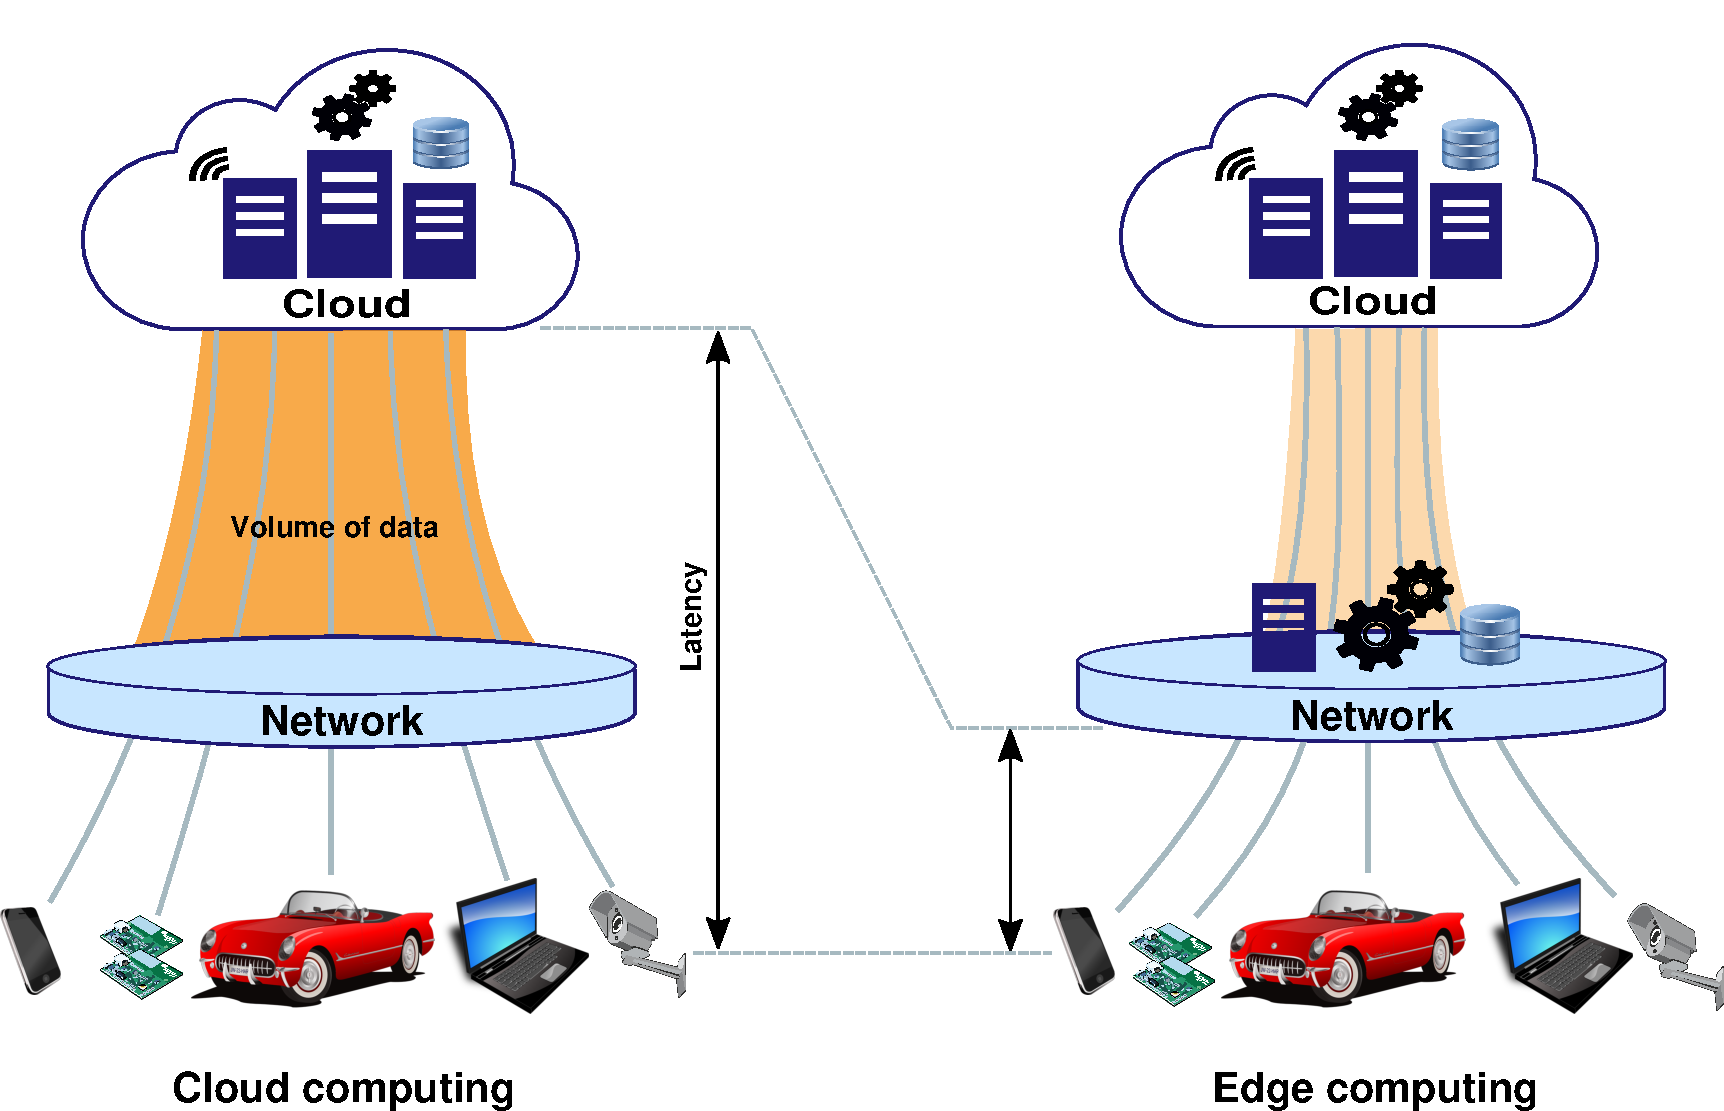
\includegraphics[width=\textwidth]{img/edge-arch.pdf}
    \end{column}
\end{columns}

\end{frame}

%-------------------------------------------------------
\section{Serverless}
\begin{frame}{Content}{}
\tableofcontents[currentsection]
\end{frame}
%-------------------------------------------------------

\begin{frame}{Serverless}{}

\begin{itemize}
    \item Promises: Abstraction from hardware and deployment specifics
  
    \item Limitations
  \begin{itemize}
      \item Stateless
      \item Requires different development approach \& tools
  \end{itemize}
  \item On the cloud:
  \begin{itemize}
    \item ``Infinite'' resources
    \item Decrease waste of resources
    \item Pay-per-use model
  \end{itemize}
  \item On the edge:
  \begin{itemize}
    \item Eases development for different hardware configurations
  \end{itemize}


\end{itemize}
\end{frame}

%-------------------------------------------------------
\section{Edge Solutions from Public Cloud Providers}
\begin{frame}{Content}{}
\tableofcontents[currentsection]
\end{frame}
%-------------------------------------------------------
\subsection{Amazon Web Services}
\renewcommand{\logofile}{img/aws}
\renewcommand{\logoscale}{0.7}
\begin{frame}{Amazon Web Services}{Edge Solutions from Public Cloud Providers}
\begin{block}{AWS Greengrass Core}
  \begin{itemize}
    \item Focuses on:
    \begin{itemize}
        \item Processing data of IoT devices
        \item Machine learning inference
    \end{itemize}
    \item Device management using AWS Greengrass IoT, features include:
    \begin{itemize}
        \item Update source code
        \item Roll out firmware upgrades
        \item Device health monitoring
    \end{itemize}
    \item Runs on low-powered devices, minimum requirements:
    \begin{itemize}
        \item 1 GHz CPU (ARM and x86)
        \item 256 MB RAM
    \end{itemize}
    \item Supports automatic data synchronization on intermittent connections
    \item Cost around \$0.20 per device per month
  \end{itemize}
  
\end{block}
\end{frame}

%-------------------------------------------------------
\subsection{Microsoft Azure}
\renewcommand{\logofile}{img/azure}
\renewcommand{\logoscale}{0.9}
\begin{frame}{Microsoft Azure}{Edge Solutions from Public Cloud Providers}

\begin{block}{Microsoft Azure IoT Edge}
  \begin{itemize}
    \item Focuses on:
    \begin{itemize}
        \item Data processing pipelines on the edge
        \item Machine learning inference
    \end{itemize}
    \item Constructs pipelines of separate modules
    \item Each module is a Docker container
    \item Minimum hardware requirements:
    \begin{itemize}
        \item Linux: x64 or ARM
        \item Windows: x64 with 2GB RAM
    \end{itemize}
    \item Supports automatic data synchronization on intermittent connections
    \item Only billed for usage of cloud resources
  \end{itemize}
\end{block}
\end{frame}

%-------------------------------------------------------
\subsection{Google Cloud}
\renewcommand{\logofile}{img/gcp}
\renewcommand{\logoscale}{0.7}
\begin{frame}{Google Cloud}{Edge Solutions from Public Cloud Providers}

\begin{block}{Google Cloud IoT}
  \begin{itemize}
    \item Mainly focuses on machine learning inference
    \item Machine learning models are trained in the cloud
    \item Supports GPU and TPU hardware acceleration
    \item Billed for data exchanges with the cloud
  \end{itemize}
\end{block}
\end{frame}
     
%-------------------------------------------------------
\subsection{IBM Cloud}
\renewcommand{\logofile}{img/ibm_cloud_functions}
\renewcommand{\logoscale}{1}
\begin{frame}{IBM Cloud}{Edge Solutions from Public Cloud Providers}

\begin{block}{Watson IoT Edge Analytics}
\begin{itemize}
    \item Relays data from IoT devices to Watson
    \item Not used for edge computing
\end{itemize}
\end{block}

\begin{block}{Apache OpenWhisk}
\begin{itemize}
    \item Open source serverless framework
    \item Made by IBM for IBM Cloud Functions
\end{itemize}
\end{block}
\end{frame}

%-------------------------------------------------------
\section{Serverless Edge Computing}
\renewcommand{\logoscale}{0}
\begin{frame}{Content}{}
\tableofcontents[currentsection]
\end{frame}

%-------------------------------------------------------
\subsection{AWS Greengrass}
\renewcommand{\logofile}{img/aws_lambda}
\renewcommand{\logoscale}{0.55}
\begin{frame}{AWS Lambda on AWS Greengrass}{Serverless Edge Computing}

\begin{block}{AWS Lambda}
\begin{itemize}
    \item Uses regular AWS Lambda functions with AWS Greengrass SDK
    \item Managed in the regular AWS Lambda interface
    \item Deployed using AWS Greengrass IoT
\end{itemize}
\end{block}
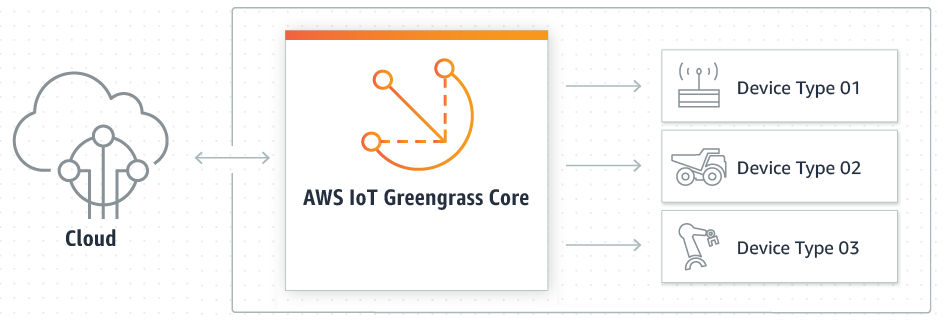
\includegraphics[width=\textwidth]{img/aws_ggc_working}\footnote{Adapted from \href{https://aws.amazon.com/greengrass/}{https://aws.amazon.com/greengrass/}}
\end{frame}

%-------------------------------------------------------
\subsection{Microsoft Azure IoT Edge}
\renewcommand{\logofile}{img/azure_functions}
\renewcommand{\logoscale}{0.7}
\begin{frame}{Azure Functions on Microsoft Azure IoT Edge}{Serverless Edge Computing}

\begin{block}{Azure Functions}
\begin{itemize}
    \item In ``Public Preview''
    \item Released open-source under the MIT licence
    \item Functions are build and deployed using Docker containers
\end{itemize}
\end{block}
\begin{figure}
    \includegraphics<2>[width=.65\textwidth]{img/install-edge-1}
    \includegraphics<3>[width=.65\textwidth]{img/install-edge-2}
    \includegraphics<4>[width=.65\textwidth]{img/install-edge-3}
    \includegraphics<5>[width=.65\textwidth]{img/install-edge-4}
    \footnote<2-5>{Adapted from https://docs.microsoft.com/en-us/azure/iot-edge/quickstart}
\end{figure}
\end{frame}

%-------------------------------------------------------
% \subsection{IBM Cloud Functions and Apache OpenWhisk}
% \begin{frame}{IBM Cloud Functions and Apache OpenWhisk}{Serverless Edge Computing}

% \begin{block}{}
% The theme contains 4 source files:
%   \begin{itemize}
%     \item 
%   \end{itemize}
% \end{block}
% \end{frame}

%-------------------------------------------------------

\section{Conclusion}
% \renewcommand{\logofile}{img/gcp}
\renewcommand{\logoscale}{0}
\begin{frame}{Conclusion}
  \begin{itemize}
      \item Edge computing solutions by public cloud providers are emerging
      \item Several mature options are already in use
      \item Two also support serverless at the edge
      \begin{itemize}
          \item AWS Greengrass
          \item Microsoft Azure IoT
      \end{itemize}
      \item Get started today!
      \begin{itemize}
          \item Each platform has a free trial/developer option
      \end{itemize}
  \end{itemize}
  
  \pause
  
  \Huge Questions?
  
\end{frame}

\end{document}